\documentclass{beamer}
\usefonttheme[onlymath]{serif}
\usepackage[T1]{fontenc}
\usepackage[utf8]{inputenc}
\usepackage[english]{babel}
\usepackage{amsmath}
\usepackage{amssymb}
\usepackage{amsthm}
\usepackage{gensymb}
\usepackage{parskip}
\usepackage{mathtools}
\usepackage{listings}
\usepackage{hyperref}
\usepackage{graphicx}
\usepackage{color}
\usepackage{enumerate}
\usepackage{tikz}
\usetikzlibrary{calc}
\usetikzlibrary{positioning}
\usetikzlibrary{angles}
\usetikzlibrary{shapes}
\usetikzlibrary{arrows}
\usepackage{verbatim}
\usepackage{multicol}
\usepackage{array}
\usepackage{minted}
\parskip 0pt


\DeclareMathOperator{\lcm}{lcm}
\newcommand\floor[1]{\left\lfloor#1\right\rfloor}
\newcommand\ceil[1]{\left\lceil#1\right\rceil}
\newcommand\abs[1]{\left|#1\right|}
\newcommand\p[1]{\left(#1\right)}
\newcommand\sqp[1]{\left[#1\right]}
\newcommand\cp[1]{\left\{#1\right\}}
\newcommand\norm[1]{\left\lVert#1\right\rVert}
\renewcommand\Im{\operatorname{Im}}
\renewcommand\Re{\operatorname{Re}}

\usetheme{metropolis}
\definecolor{dark yellow}{rgb} {0.6,0.6,0.0}
\definecolor{dark green}{rgb} {0.0,0.6,0.0}

\graphicspath{{myndir/}}

\title{Heap}
\author{Arnar Bjarni Arnarson}
\institute{\href{http://ru.is/td}{School of Computer Science} \\[2pt] \href{http://ru.is}{Reykjavík University}}
\titlegraphic{\hfill\includegraphics[height=0.6cm]{kattis}}

\begin{document}
\maketitle

\begin{frame}[plain]{Heaps}
    \begin{itemize}
        \item<1-> As an example of a data structure in the standard library but that sometimes requires a more powerful version, let us consider heaps.
        \item<2-> Heaps are implemented in most standard libraries in the forms of priority queues.
        \item<3-> A heap is nothing but a binary tree satisfying \textit{the heap condition}.
        \item<4-> The heap condition (for a min heap) says that the value of any given node is not greater than that of its children.
    \end{itemize}
\end{frame}

\begin{frame}[plain]{Heaps}
    \begin{itemize}
        \item<1-> Since arrays are linear, we want to smush this binary tree into an array for the implementation.
        \item<2-> We can do this by putting the root at index $1$.
        \item<2-> Then the children of item at index $i$ are simply at $2i$ and $2i+1$.
        \item<2-> The parent of any item $i > 1$ is then $\floor{\frac{i}{2}}$.
        \item<3-> We could do this using raw arrays (then index $0$ can be used to store its size), but the examples will be given in C++ using vectors.
    \end{itemize}
\end{frame}

\begin{frame}[plain]{Heaps}
    \begin{center}
    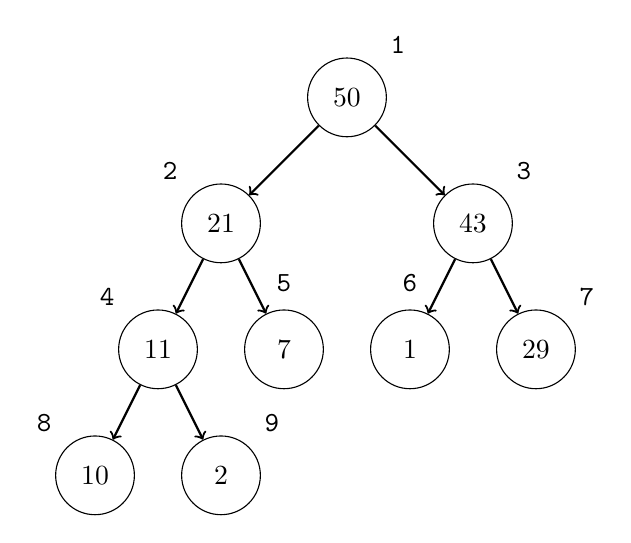
\begin{tikzpicture}[scale=0.8]
    \def\spa{2}
    \node[minimum size=1cm, draw, circle] (A) at (0, 0) {$50$};
    \node[minimum size=1cm, draw, circle] (B) at (-\spa, -\spa) {$21$};
    \node[minimum size=1cm, draw, circle] (C) at (\spa, -\spa) {$43$};
    \node[minimum size=1cm, draw, circle] (D) at (-1.5*\spa, -2*\spa) {$11$};
    \node[minimum size=1cm, draw, circle] (E) at (-0.5*\spa, -2*\spa) {$7$};
    \node[minimum size=1cm, draw, circle] (F) at (0.5*\spa, -2*\spa) {$1$};
    \node[minimum size=1cm, draw, circle] (G) at (1.5*\spa, -2*\spa) {$29$};
    \node[minimum size=1cm, draw, circle] (H) at (-2*\spa, -3*\spa) {$10$};
    \node[minimum size=1cm, draw, circle] (I) at (-\spa, -3*\spa) {$2$};
    
    \node (Ai) [above right=0.1cm of A] {\texttt{1}};
    \node (Bi) [above left=0.1cm of B] {\texttt{2}};
    \node (Ci) [above right=0.1cm of C] {\texttt{3}};
    \node (Di) [above left=0.1cm of D] {\texttt{4}};
    \node (Ei) [above=0.1cm of E] {\texttt{5}};
    \node (Fi) [above=0.1cm of F] {\texttt{6}};
    \node (Gi) [above right=0.1cm of G] {\texttt{7}};
    \node (Hi) [above left=0.1cm of H] {\texttt{8}};
    \node (Ii) [above right=0.1cm of I] {\texttt{9}};
    
    \draw[->, thick] (A) -- (B);
    \draw[->, thick] (A) -- (C);
    \draw[->, thick] (B) -- (D);
    \draw[->, thick] (B) -- (E);
    \draw[->, thick] (C) -- (F);
    \draw[->, thick] (C) -- (G);
    \draw[->, thick] (D) -- (H);
    \draw[->, thick] (D) -- (I);
    \end{tikzpicture}
    \end{center}
    \begin{large}
    \texttt{ARRAY: [SIZE, 50, 21, 43, 11, 7, 1, 29, 10, 2]}
    \end{large}
\end{frame}

\begin{frame}[plain]{Heaps}
    \begin{itemize}
        \item<1->Items can be inserted by pushing them to the back and fixing the heap condition upwards from them.
        \item<2-> Items can be deleted by replacing the smallest value with a leaf and then fixing the heap condition downwards.
        \item<3-> Let us see how this would look in C++.
    \end{itemize}
\end{frame}

\begin{frame}[plain, fragile]{C++ implementation (min-heap)}
    \scriptsize
    \begin{minted}{cpp}
template<typename T> struct Heap {
    vector<T> h; Heap() : h(1) { }
    constexpr size_t size() { return h.size() - 1; }
    constexpr T peek() { return h[1]; }
    void swim(size_t i) {
        while(i != 1 && h[i] < h[i / 2]) {
            swap(h[i], h[i / 2]);
            i /= 2; } }
    void sink(size_t i) {
        while(true) {
            size_t mn = i;
            if(2 * i + 1 < h.size() && h[mn] > h[2 * i + 1]) mn = 2 * i + 1;
            if(2 * i  < h.size() && h[mn] > h[2 * i]) mn = 2 * i;
            if(mn != i) swap(h[i], h[mn]), i = mn;
            else break; } }
    void pop() {
        h[1] = h.back();
        h.pop_back(); sink(1); }
    void push(T x) {
        h.push_back(x);
        swim(h.size() - 1); } };
    \end{minted}
\end{frame}

\begin{frame}[plain]{Heaps}
    \begin{itemize}
        \item<1-> We note that peek and size run in $\mathcal{O}(1)$ while all other operations run in $\mathcal{O}(log(n))$.
        \item<2-> This implementation isn't any better than the standard library one in C++.
        \item<3-> We provide it for demonstration of representing binary trees with an array.
    \end{itemize}
\end{frame}

\end{document}
